%%%%%%%%%%%%%%%%%%%%%%%%%%%%%%
% AAAI Presentation!!
% Made using Karl Broman's guide:
% https://kbroman.org/blog/2013/10/07/better-looking-latexbeamer-slides/
% 

\documentclass[12pt,t]{beamer}
\usepackage{fontspec}
\setmainfont{Optima Medium.ttf}

%═══════════════════════════════════════════
% Math packages
%═══════════════════════════════════════════
\usepackage{amssymb,amsthm,amsmath}
\usepackage{mathtools}
\usepackage{proof}
\usepackage{bussproofs}
\usepackage{marvosym}

%═══════════════════════════════════════════
% Environments
%═══════════════════════════════════════════
\theoremstyle{definition}

% \newtheorem{theorem}{Theorem}

% \newtheorem{definition}{Definition}
% \newtheorem{lemma}[theorem]{Lemma}
% \newtheorem{claim}{Claim}
% \newtheorem{corollary}{Corollary}
% \newtheorem{proposition}{Proposition}
% \newtheorem{example}{Example}
% \newtheorem{remark}[theorem]{Remark}
% \newenvironment{sketch}{\begin{proof}[Proof Sketch]}{\end{proof}}

\usepackage{lmodern}
\makeatletter
\setbeamertemplate{theorem begin}{
  {
    \hilight{\bfseries \textup{\inserttheoremname.}}
    \ifx\inserttheoremaddition\@empty\else\ (\inserttheoremaddition)\fi%
    \space% new
  }
}

\setbeamertemplate{theorem end}{}
\makeatother

%═══════════════════════════════════════════
% Graphics packages
%═══════════════════════════════════════════
\usepackage{tikz}
\usepackage{graphicx}
\usetikzlibrary{positioning,calc,arrows.meta,shapes.geometric,fit, backgrounds, external}
\tikzexternalize
\usepackage{tabularx}

%═══════════════════════════════════════════
% Custom Commands, General Use
%═══════════════════════════════════════════
\newcommand{\key}[1]{\emph{#1}}
\newcommand{\Rat}{\mathbb{Q}}
\newcommand{\Nat}{\mathbb{N}}
\newcommand{\State}{\mathsf{State}} 
\newcommand{\semantics}[1]{[\![\mbox{\em $ #1 $\/}]\!]}
\newcommand{\Model}{\mathcal{M}}
\newcommand{\Nodel}{\mathcal{N}}
\newcommand{\lang}{\mathcal{L}}
\newcommand{\uplang}{\mathcal{L}^\ast}
\newcommand{\vocab}{\mathcal{V}}
\newcommand{\wocab}{\mathcal{W}}
\newcommand{\set}[1]{\{ #1 \}}
\newcommand{\proves}{\vdash}
\renewcommand{\o}{\cdot}
\newcommand{\orr}{\vee}
\newcommand{\andd}{\wedge}
\newcommand{\nott}{\neg}
\newcommand{\bigandd}{\bigwedge}
\newcommand{\quadiff}{\quad \mbox{ iff } \quad}
\newcommand{\rem}[1]{\relax}
 \newcommand{\NP}{\mbox{\sc np}}
\newcommand{\axiom}{\textsc}
\newcommand*{\bigchi}{\mbox{\Large$\chi$}}% big chi
\newcommand{\degree}[1]{\mathrm{deg}(#1)}
\newcommand{\preds}[1]{\mbox{preds}(#1)}
\newcommand{\layer}[1]{\mathsf{layer}(#1)}
\newcommand{\activ}[2]{\mathsf{activ}_{#1}(#2)}
\newcommand{\layerNoArgs}{\mathsf{layer}}

\newcommand{\negweightscore}[1]{\mathsf{nws}(#1)}
\newcommand{\minscore}{\mathsf{mnws}}
\newcommand{\numiterations}{\mathsf{iter}}

%═══════════════════════════════════════════
% Custom Commands, Hebbian Learning
%═══════════════════════════════════════════
\newcommand{\AllNets}{\mathsf{Net}}
\newcommand{\Net}{\mathcal{N}}
\newcommand{\op}{\mathsf{op}}
\newcommand{\Best}{\mathsf{Best}}
\newcommand{\Prop}{\mathsf{Prop}}
\newcommand{\Reach}{\mathsf{Reach}}
\newcommand{\Hebb}[2]{\mathsf{Hebb}(#1, #2)}
\newcommand{\HebbNoArgs}{\mathsf{Hebb}}
\newcommand{\Hebbstar}[2]{\mathsf{Hebb}^*(#1, #2)}
\newcommand{\HebbstarNoArgs}{\mathsf{Hebb}^*}
\newcommand{\hebbweight}{W_\mathsf{Hebb}}
\newcommand{\hebbstarweight}{W_{\mathsf{Hebb}^*}}

\newcommand{\Typ}[1]{\textrm{\textup{\textbf{T}}} #1}
\newcommand{\Know}[1]{\textrm{\textup{\textbf{K}}} #1}
% \newcommand{\Know}[2]{\textrm{\textup{\textbf{K}}}(#1, #2)}
\newcommand{\KnowNoArgs}{\textrm{\textup{\textbf{K}}}}
\newcommand{\TypNoArgs}{\textrm{\textup{\textbf{T}}}}
% \newcommand{\Hebbop}[1]{[#1]_\textrm{\textup{hebb}\:}}
% \newcommand{\Hebbop}[1]{[#1]_{\HebbstarNoArgs}\:}
\newcommand{\Hebbop}[1]{[#1]}

\newcommand{\diaTyp}[1]{\langle \textrm{\textup{\textbf{T}}} \rangle #1}
\newcommand{\diaKnow}[1]{\langle \textrm{\textup{\textbf{K}}} \rangle #1}
% \newcommand{\diaKnow}[2]{\langle \textrm{\textup{\textbf{K}}} \rangle(#1, #2)}
\newcommand{\diaTypNoArgs}{\langle \textrm{\textup{\textbf{T}}} \rangle}
\newcommand{\diaKnowNoArgs}{\langle \textrm{\textup{\textbf{K}}} \rangle}
% \newcommand{\diaHebbop}[1]{\langle #1\rangle_\textrm{\textup{hebb}}}
\newcommand{\diaHebbop}[1]{\langle #1\rangle}



\usepackage[absolute,overlay]{textpos}
\usepackage{tikz}
\usepackage{caption}

\usepackage[style=verbose,backend=biber,giveninits=true]{biblatex}
\addbibresource{neurosymbolic.bib}
\ExecuteBibliographyOptions{isbn=false,url=false,doi=false,eprint=false}
\AtEveryCitekey{\clearfield{pages}} 

%%%%%%%%%%%%%%%%%%%%%%%%%%%%%%
% Title Setup
\setbeamertemplate{frametitle}{\vspace{1ex} \bfseries \centerline{ \insertframetitle}}

%%%%%%%%%%%%%%%%%%%%%%%%%%%%%%
% Setup for notes
% \setbeameroption{hide notes}
% \setbeamertemplate{note page}[plain]

%%%%%%%%%%%%%%%%%%%%%%%%%%%%%%
% Set default Beamer theme,
% get rid of navigation, and
% disable bookmarks when opening
% in Acrobat.
\usetheme{default}
\beamertemplatenavigationsymbolsempty{}
\hypersetup{pdfpagemode=UseNone} % Don't show bookmarks when viewing in Acrobat

% \usefonttheme{professionalfonts}
% \usefonttheme{serif}
% \setmainfont{TeX Gyre Pagella}
% \setbeamerfont{note page}{family*=pplx,size=\footnotesize} % Palatino for notes

% \usefonttheme{professionalfonts}
% \usefonttheme{serif}
% \usepackage{fontspec}
% %\setmainfont{Helvetica Neue}
% \setmainfont{TeX Gyre Heros}
% \setbeamerfont{note page}{family*=pplx,size=\footnotesize} % Palatino for notes

% \definecolor{background}{HTML}{fbf1c7}
% \definecolor{gruvgreen}{HTML}{79740e}
% \definecolor{gruvblue}{HTML}{076678}
% \definecolor{gruvpurple}{HTML}{8f3f71}
% \definecolor{gruvyellow}{HTML}{d79921} % b57614
% \definecolor{gruvred}{HTML}{9d0006}
% \definecolor{gruvblack}{HTML}{3c3836}
% \definecolor{gruvgrey}{HTML}{ebdbb2} %7c6f64

% Gruvbox Colors
\definecolor{foreground}{HTML}{3c3836}
\definecolor{background}{HTML}{f9f5d7} %fbf1c7
\definecolor{gray}{HTML}{7c6f64}

\definecolor{title}{HTML}{9d0006}
\definecolor{institute}{HTML}{3c3836}
\definecolor{subtitle}{HTML}{8f3f71}
\definecolor{hilight}{HTML}{8f3f71}
\definecolor{gruvgreen}{HTML}{79740e}
\definecolor{gruvblue}{HTML}{076678}

%%%%%%%%%%%%%%%%%%%%%%%%%%%%%%
% Establish that these are the
% colors we are using.
\setbeamercolor{titlelike}{fg=title}
\setbeamercolor{subtitle}{fg=subtitle}
\setbeamercolor{institute}{fg=institute}
\setbeamercolor{normal text}{fg=foreground,bg=background}
\setbeamercolor{block title}{fg=title}
% \setbeamercolor{note page}{bg=background}

%%%%%%%%%%%%%%%%%%%%%%%%%%%%%%
% Change the color of bullets
% in itemize environments and change
% the style of nested bullets to - dashes
\setbeamercolor{item}{fg=foreground} % color of bullets
\setbeamercolor{subitem}{fg=gray}
\setbeamercolor{itemize/enumerate subbody}{fg=gray}
\setbeamertemplate{itemize items}[circle]
\setbeamertemplate{itemize subitem}{{\textendash}}
\setbeamerfont{itemize/enumerate subbody}{size=\footnotesize}
\setbeamerfont{itemize/enumerate subitem}{size=\footnotesize}
\setbeamerfont{footnote}{size=\tiny}
\setbeamertemplate{bibliography item}{}

%%%%%%%%%%%%%%%%%%%%%%%%%%%%%%
% Change the color of citations
\setbeamercolor{bibliography entry author}{fg=hilight}
\setbeamercolor{bibliography entry title}{fg=foreground}
\setbeamercolor{bibliography entry note}{fg=gray}

%%%%%%%%%%%%%%%%%%%%%%%%%%%%%%
% Number the slides in the lower-right
\setbeamertemplate{footline}{%
    \raisebox{5pt}{\makebox[\paperwidth]{\hfill\makebox[20pt]{\color{gray}
          \scriptsize\insertframenumber}}}\hspace*{5pt}}

\renewcommand*\footnoterule{}

%%%%%%%%%%%%%%%%%%%%%%%%%%%%%%          
% Separate paragraphs on the notes page
% \addtobeamertemplate{note page}{\setlength{\parskip}{12pt}}

%%%%%%%%%%%%%%%%%%%%%%%%%%%%%%%%%%%%%%%%%%%
% Presentation macros
\newcommand{\bi}{\begin{itemize}}
\newcommand{\ib}{\end{itemize}}
\newcommand{\graphic}{\includegraphics}
\newcommand{\subt}[1]{{\footnotesize \color{subtitle} {#1}}}
\newcommand{\hilight}[1]{\color{hilight} #1}

\usepackage[super]{nth}

%\bibliographystyle{abbrv}
% \bibliography{main}

\title{\Large{\textbf{Logical Dynamics of\\ Neural Network Learning}}}
\author{ \large{\hilight{\textbf{Caleb Schultz Kisby}}}
}
\institute{\normalsize{Collab.\ with Sa\'ul Blanco \& Larry Moss\\ Indiana University}}
\date{\nth{1} GALAI Workshop\\ \today}


% For notes on second screen
% \usepackage{pgfpages}
% \makeatletter 
% \def\beamer@framenotesbegin{% at beginning of slide
%      \usebeamercolor[fg]{normal text}
%       \gdef\beamer@noteitems{}% 
%       \gdef\beamer@notes{}%
% }
% \makeatother

\begin{document}

%\setbeameroption{show notes}
% \setbeameroption{show notes on second screen=right}
% \setbeamerfont{note page}{size=\scriptsize}

%%%%%%%%%%%%%%%%%%%%%%%%%%%%%%%%%%%%%%%%
% Title Slide
{
\setbeamertemplate{footline}{} % no page number here

%------------------------------------------------
\frame{
    \titlepage
}}

%------------------------------------------------
\begin{frame}{Foundations for Neuro-Symbolic AI}
% \vspace{1ex}

From van Harmelen (2022):\footcite{vanHarmelen}\\
\vspace{1ex}

\begin{quote}
    \footnotesize \textup{``What are the possible interactions between knowledge and learning? Can reasoning be used as a symbolic prior for learning $\ldots$ Can symbolic constraints be enforced on data-driven systems to make them safer? Or less biased? Or can, vice versa, learning be used to yield symbolic knowledge? And if so, how to manage the inherent uncertainty that comes with such learned knowledge$\ldots$''}
\end{quote}

% He continues:\\
\vspace{1ex}

\begin{quote}
    \footnotesize \textup{``$\ldots$ neuro-symbolic systems currently lack a theory that even begins to ask these questions, let alone answer them. All too often, new conference papers and ArXiv manuscripts simply propose a new neuro-symbolic architecture, or a new algorithm, without even discussing which of the above questions (or any others, for that matter) they aim to address.''}
\end{quote}


\end{frame}

%------------------------------------------------
\begin{frame}{Neural Network Semantics}
\vspace{1ex}
\centering
\pause
% $P, Q \in p \mid P \land Q \mid \varphi \to \psi$\\
% Formulas: $P \Rightarrow Q$\\
% \vspace{2ex}

% \begin{columns}
% \begin{column}{0.45\textwidth}
%     $\Model = \langle W, R, \prec, V \rangle$
%     \vspace{1ex}
    
%     $\Best_\Model(S) =$\\
%     \quad \quad $\{ w \mid \forall u \in S, w \prec u\}$
    
% \end{column}
% \vrule \quad
% \begin{column}{0.45\textwidth}
    $\Net = \langle N, E, W, A, \eta, \semantics{\cdot} \rangle$
    \vspace{1ex}\\

    $\Prop_\Net(S): \mathcal{P}(N) \to \mathcal{P}(N)$
    \vspace{1ex}\\

    $\Prop_\Net(S) =$ the set of all nodes that are\\ eventually activated on input $S$
    \vspace{2ex}
    
    \includegraphics{fig-prop.pdf}

    \vspace{2ex}
    $\Net \models \varphi \Rightarrow \psi$ iff $\Prop_\Net(\semantics{\varphi}) \supseteq \semantics{\psi}$
% \end{column}
% \end{columns}

\end{frame}

\begin{frame}{A Brief Timeline}
\vspace{1ex}
\centering

\begin{description}
    \item[1991.] Balkenius \& G{\"a}rdenfors realize that $\Prop$ behaves like a nonmonotonic conditionals
    \item[2001.] Leitgeb proves this, via a completeness theorem
    \item[2003.] Leitgeb extends completeness to various neural network architectures
    \item[2022.] Giordano, Gliozzi, \& Theseider Dupré prove soundness for fuzzy activation functions
    \item[2022.] Schultz Kisby, Blanco, \& Moss prove soundness for a basic learning policy (Hebbian learning)
    \item[2022.] Odense \& d’Avila Garcez start writing a survey of approaches like this (they call this ``semantic encoding'')
    \item[2024.] Our new result: Completeness for Hebbian Learning!  (Accepted paper at AAAI 2024)
\end{description}

\end{frame}



%------------------------------------------------
\begin{frame}{Soundness \& Completeness}
\vspace{1ex}
\begin{itemize}
\item Leitgeb (2001)\footcite{leitgeb2001nonmonotonic} showed that the neural semantics for $\varphi \Rightarrow \psi$ are completely axiomatized by:
\vspace{1ex}
\begin{description}
    \item[Refl.] $\varphi \Rightarrow \varphi$
    \item[LLE.] $\frac{\varphi \leftrightarrow \psi \quad \varphi \Rightarrow \rho}{\psi \Rightarrow \rho}$
    \item[Weak.] $\frac{\varphi \to \psi \quad \rho \Rightarrow \varphi}{\rho \Rightarrow \psi}$
    \item[CC.] $\frac{\varphi \land \psi \Rightarrow \rho \quad \varphi \Rightarrow \psi}{\varphi \Rightarrow \rho}$
    \item[CM.] $\frac{\varphi \Rightarrow \psi \quad \varphi \Rightarrow \rho}{\varphi \land \psi \Rightarrow \rho}$
    \item[Loop.] $\frac{\varphi_0 \Rightarrow \varphi_1 \quad \ldots \varphi_{k-1} \Rightarrow \varphi_{k} \quad \varphi_k \Rightarrow \varphi_0}{\varphi_i \Rightarrow \varphi_j}$
\end{description}

\vspace{1ex}
\item This is classified as a ``Loop-Cumulative'' conditional by Kraus, Lehmann, and Magidor (1990)\footcite{kraus1990nonmonotonic}
\end{itemize}
\end{frame}

%------------------------------------------------
\begin{frame}{Learning Wrecks the Model!}
    \vspace{1ex}
\centering

\vspace{12ex}
[See board]

\end{frame}

%------------------------------------------------
\begin{frame}{Hebbian Learning}
\vspace{1ex}
\centering

\emph{Neurons that fire together wire together}
\vspace{2ex}

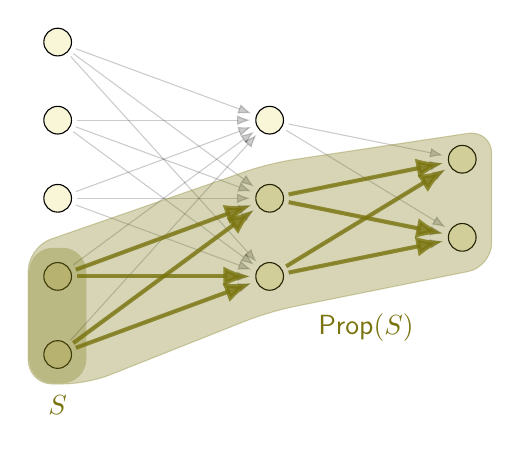
\begin{tikzpicture}[loose/.style={inner sep=.7em},edge/.style = {->,-Latex},
    oval/.style={ellipse,draw}]

    %--------------------------------------------
    % Nodes
    \node[circle,minimum size=10pt,inner sep=0pt,outer sep=2pt,fill=background,draw](a){};
    
    \node[below=0.5 of a,circle,minimum size=10pt,inner sep=0pt,outer sep=2pt,fill=background,draw](b){};
    
    \node[below=0.5 of b,circle,minimum size=10pt,inner sep=0pt,outer sep=2pt,fill=background,draw](c){};
    
    \node[below=0.5 of c,circle,minimum size=10pt,inner sep=0pt,outer sep=2pt,fill=background,draw](d){};
    
    \node[below=0.5 of d,circle,minimum size=10pt,inner sep=0pt,outer sep=2pt,fill=background,draw](e){};
    
    \node[right=2.2 of b,circle,minimum size=10pt,inner sep=0pt,outer sep=2pt,fill=background,draw](f){};
    
    \node[right=2.2 of c,circle,minimum size=10pt,inner sep=0pt,outer sep=2pt,fill=background,draw](g){};
    
    \node[right=2.2 of d,circle,minimum size=10pt,inner sep=0pt,outer sep=2pt,fill=background,draw](h){};
    
    \node[right=2.2 of $(f)!0.5!(g)$,circle,minimum size=10pt,inner sep=0pt,outer sep=2pt,fill=background,draw](i){};

    \node[right=2.2 of $(g)!0.5!(h)$,circle,minimum size=10pt,inner sep=0pt,outer sep=2pt,fill=background,draw](j){};
    
    %--------------------------------------------
    % The set S
    \node[fill=gruvgreen, color=gruvgreen, very thick, opacity=0.3,rectangle,rounded corners=2ex,fit=(d) (e)]{};

    \node [color=gruvgreen,opacity=1,below=0.4 of $(e)$]{$S$};
    
    %--------------------------------------------
    % Edges
    % How to color an edge:
    % \draw[edge, line width=1.5pt, color=gruvgreen, opacity=0.8] (a) to (g);
    \draw[edge, color=black, opacity=0.2] (a) -- (f) node [near start, above] {};
    \draw[edge, color=black, opacity=0.2] (a) -- (g) node [near start, above] {};
    \draw[edge, color=black, opacity=0.2] (a) -- (h) node [near start, above] {};
    
    \draw[edge, color=black, opacity=0.2] (b) -- (f) node [near start, above] {};
    \draw[edge, color=black, opacity=0.2] (b) -- (g) node [near start, above] {};
    \draw[edge, color=black, opacity=0.2] (b) -- (h) node [near start, above] {};

    \draw[edge, color=black, opacity=0.2] (c) -- (f) node [near start, above] {};
    \draw[edge, color=black, opacity=0.2] (c) -- (g) node [near start, above] {};
    \draw[edge, color=black, opacity=0.2] (c) -- (h) node [near start, above] {};

    \draw[edge, color=black, opacity=0.2] (d) -- (f) node [near start, above] {};
    \draw[edge, color=black, opacity=0.2] (e) -- (f) node [near start, above] {};
    \draw[edge, color=black, opacity=0.2] (f) -- (i) node [near start, above] {};
    \draw[edge, color=black, opacity=0.2] (f) -- (j) node [near start, above] {};
    
    % These edges disappear
    \only<1-2>{
    \draw[edge, color=black, opacity=0.2] (d) -- (g) node [near start, above] {};
    \draw[edge, color=black, opacity=0.2] (d) -- (h) node [near start, above] {};
    
    \draw[edge, color=black, opacity=0.2] (e) -- (g) node [near start, above] {};
    \draw[edge, color=black, opacity=0.2] (e) -- (h) node [near start, above] {};
    
    \draw[edge, color=black, opacity=0.2] (g) -- (i) node [near start, above] {};
    \draw[edge, color=black, opacity=0.2] (h) -- (i) node [near start, above] {};
    
    \draw[edge, color=black, opacity=0.2] (g) -- (j) node [near start, above] {};
    \draw[edge, color=black, opacity=0.2] (h) -- (j) node [near start, above] {};
    }
    %------------------------------------------------------------
    % FRAME 2
    % The propagation of S
    \draw[fill=gruvgreen, color=gruvgreen, opacity=0.3, rounded corners=2ex] 
    ([xshift=-0.2cm,yshift=0.2cm] d.north west)
    -- ([yshift=0.2cm] g.north)
    -- ([xshift=0.2cm, yshift=0.2cm] i.north east)
        
    -- ([xshift=0.2cm,yshift=-0.2cm] j.south east)
    -- ([yshift=-0.2cm] h.south)
    -- ([xshift=0.2cm,yshift=-0.2cm] e.south east)
    -- ([xshift=-0.2cm,yshift=-0.2cm] e.south west)
    -- cycle;
    
    \node [color=gruvgreen,opacity=1, below=0.6 of $(h)!0.5!(j)$]{$\Prop(S)$};
    

    %------------------------------------------------------------
    % FRAME 3
    
    \draw[edge, line width=1.5pt, color=gruvgreen, opacity=0.8] (d) to (g);
    \draw[edge, line width=1.5pt, color=gruvgreen, opacity=0.8] (d) to (h);
    \draw[edge, line width=1.5pt, color=gruvgreen, opacity=0.8] (e) to (g);
    \draw[edge, line width=1.5pt, color=gruvgreen, opacity=0.8] (e) to (h);
    \draw[edge, line width=1.5pt, color=gruvgreen, opacity=0.8] (g) to (i);
    \draw[edge, line width=1.5pt, color=gruvgreen, opacity=0.8] (h) to (i);
    \draw[edge, line width=1.5pt, color=gruvgreen, opacity=0.8] (g) to (j);
    \draw[edge, line width=1.5pt, color=gruvgreen, opacity=0.8] (h) to (j);
\end{tikzpicture}


\end{frame}

%------------------------------------------------
\begin{frame}{Iterated Hebbian Learning}
\vspace{1ex}
\centering

\emph{Neurons that fire together wire together}
\vspace{2ex}

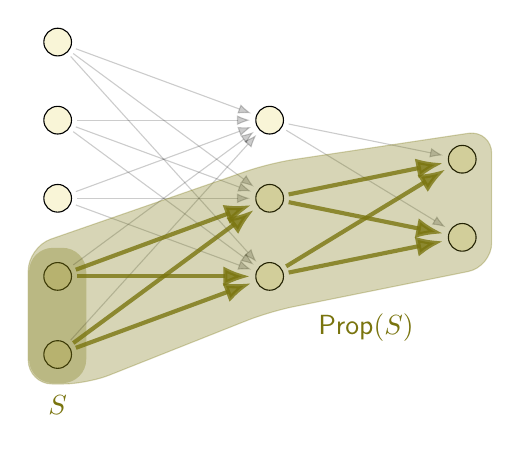
\begin{tikzpicture}[loose/.style={inner sep=.7em},edge/.style = {->,-Latex},
    oval/.style={ellipse,draw}]

    %--------------------------------------------
    % Nodes
    \node[circle,minimum size=10pt,inner sep=0pt,outer sep=2pt,fill=background,draw](a){};
    
    \node[below=0.5 of a,circle,minimum size=10pt,inner sep=0pt,outer sep=2pt,fill=background,draw](b){};
    
    \node[below=0.5 of b,circle,minimum size=10pt,inner sep=0pt,outer sep=2pt,fill=background,draw](c){};
    
    \node[below=0.5 of c,circle,minimum size=10pt,inner sep=0pt,outer sep=2pt,fill=background,draw](d){};
    
    \node[below=0.5 of d,circle,minimum size=10pt,inner sep=0pt,outer sep=2pt,fill=background,draw](e){};
    
    \node[right=2.2 of b,circle,minimum size=10pt,inner sep=0pt,outer sep=2pt,fill=background,draw](f){};
    
    \node[right=2.2 of c,circle,minimum size=10pt,inner sep=0pt,outer sep=2pt,fill=background,draw](g){};
    
    \node[right=2.2 of d,circle,minimum size=10pt,inner sep=0pt,outer sep=2pt,fill=background,draw](h){};
    
    \node[right=2.2 of $(f)!0.5!(g)$,circle,minimum size=10pt,inner sep=0pt,outer sep=2pt,fill=background,draw](i){};

    \node[right=2.2 of $(g)!0.5!(h)$,circle,minimum size=10pt,inner sep=0pt,outer sep=2pt,fill=background,draw](j){};
    
    %--------------------------------------------
    % The set S
    \node[fill=gruvgreen, color=gruvgreen, very thick, opacity=0.3,rectangle,rounded corners=2ex,fit=(d) (e)]{};

    \node [color=gruvgreen,opacity=1,below=0.4 of $(e)$]{$S$};
    
    %--------------------------------------------
    % Edges
    \draw[edge, color=black, opacity=0.2] (a) -- (f) node [near start, above] {};
    \draw[edge, color=black, opacity=0.2] (a) -- (g) node [near start, above] {};
    \draw[edge, color=black, opacity=0.2] (a) -- (h) node [near start, above] {};
    
    \draw[edge, color=black, opacity=0.2] (b) -- (f) node [near start, above] {};
    \draw[edge, color=black, opacity=0.2] (b) -- (g) node [near start, above] {};
    \draw[edge, color=black, opacity=0.2] (b) -- (h) node [near start, above] {};

    \draw[edge, color=black, opacity=0.2] (c) -- (f) node [near start, above] {};
    \draw[edge, color=black, opacity=0.2] (c) -- (g) node [near start, above] {};
    \draw[edge, color=black, opacity=0.2] (c) -- (h) node [near start, above] {};

    \draw[edge, color=black, opacity=0.2] (d) -- (f) node [near start, above] {};
    \draw[edge, color=black, opacity=0.2] (e) -- (f) node [near start, above] {};
    \draw[edge, color=black, opacity=0.2] (f) -- (i) node [near start, above] {};
    \draw[edge, color=black, opacity=0.2] (f) -- (j) node [near start, above] {};

    % The propagation of S
    \draw[fill=gruvgreen, color=gruvgreen, opacity=0.3, rounded corners=2ex] 
        ([xshift=-0.2cm,yshift=0.2cm] d.north west)
        -- ([yshift=0.2cm] g.north)
        -- ([xshift=0.2cm, yshift=0.2cm] i.north east)
        
        -- ([xshift=0.2cm,yshift=-0.2cm] j.south east)
        -- ([yshift=-0.2cm] h.south)
        -- ([xshift=0.2cm,yshift=-0.2cm] e.south east)
        -- ([xshift=-0.2cm,yshift=-0.2cm] e.south west)
        -- cycle;
    
    \node [color=gruvgreen,opacity=1, below=0.6 of $(h)!0.5!(j)$]{$\Prop(S)$};
    
    \draw[edge, line width=1.5pt, color=gruvgreen, opacity=0.8] (d) to (g);
    \draw[edge, line width=1.5pt, color=gruvgreen, opacity=0.8] (d) to (h);
    \draw[edge, line width=1.5pt, color=gruvgreen, opacity=0.8] (e) to (g);
    \draw[edge, line width=1.5pt, color=gruvgreen, opacity=0.8] (e) to (h);
    \draw[edge, line width=1.5pt, color=gruvgreen, opacity=0.8] (g) to (i);
    \draw[edge, line width=1.5pt, color=gruvgreen, opacity=0.8] (h) to (i);
    \draw[edge, line width=1.5pt, color=gruvgreen, opacity=0.8] (g) to (j);
    \draw[edge, line width=1.5pt, color=gruvgreen, opacity=0.8] (h) to (j);
\end{tikzpicture}

Repeat this update until a fixed point!\\
i.e.\ until the weights are ``maximally high''


\end{frame}

%------------------------------------------------
\begin{frame}{Language and Semantics}
\vspace{1ex}
\centering

$p \mid \neg \varphi \mid \varphi \land \psi \mid \Know{\varphi} \mid \Typ{\varphi} \mid \Hebbop{\varphi} \psi$\\

% \pause
\vspace{1ex}
We define duals $\diaKnowNoArgs$, $\diaTypNoArgs$ as usual.

% \pause
\[
    \begin{array}{lcl}
        \semantics{p} & \in & \mathcal{P}(N) \\
        \semantics{\neg \varphi} & = & \semantics{\varphi}^\complement \\
        \semantics{\varphi \land \psi} & = & \semantics{\varphi} \cap \semantics{\psi} \\

        % \pause
        \semantics{\diaKnow{\varphi}} & = & \Reach(\semantics{\varphi}) \\
        \semantics{\diaTyp{\varphi}} & = & \Prop(\semantics{\varphi})\\

        % \pause
        \semantics{\Hebbop{\varphi} \psi}_{\Net} & = & \semantics{\psi}_{\Hebb{\Net}{\semantics{\varphi}}}
    \end{array}
\]

% \pause
\vspace{1ex}
We also define $\Net \models \varphi$ iff $\semantics{\varphi}_\Net$ = N

% \pause
\vspace{2ex}
Note that we can express\\ 
Leitgeb's $\varphi \Rightarrow \psi$ as $\Typ{\varphi} \to \psi$

\end{frame}

%------------------------------------------------
\begin{frame}{Soundness for $\KnowNoArgs$ and $\TypNoArgs$}
\centering

\begin{itemize}
    \item First, $\Reach$ is a standard monotonic closure operator:
    \begin{description}
        \item[Nec.] From $\proves \varphi$ we can infer $\proves \Know{\varphi}$
        \item[Dual.] $\diaKnow{\varphi} \leftrightarrow \neg \Know{\neg \varphi}$
        \item[Refl.] $\Know{\varphi} \to \varphi$
        \item[Trans.] $\Know{\varphi} \to \Know{\Know{\varphi}}$
        \item[Distr.] $\Know{(\varphi \to \psi)} \leftrightarrow (\Know{\varphi} \to \Know{\psi})$
    \end{description}

    % \pause
    \vspace{1ex}
    \item $\Prop$ is non-monotonic, but is ``Loop-Cumulative'':
    \begin{description}
        \item[Nec.] From $\proves \varphi$ we can infer $\proves \Typ{\varphi}$
        \item[Dual.] $\diaTyp{\varphi} \leftrightarrow \neg \Typ{\neg \varphi}$
        \item[Refl.] $\Typ{\varphi} \to \varphi$
        \item[Trans.] $\Typ{\varphi} \to \Typ{\Typ{\varphi}}$
        \item[Cumulative.] $(\varphi \to \psi) \land (\Typ{\psi} \to \varphi) \to (\Typ{\varphi} \to \psi)$
        \item[Loop.] \small $(\Typ \varphi_0 \to \varphi_1) \land \cdots \land (\Typ \varphi_k \to \varphi_0) \to (\Typ \varphi_0 \to \varphi_k)$ \normalsize
    \end{description}
\end{itemize}

\end{frame}

%------------------------------------------------
\begin{frame}{A Complete Description of $\HebbstarNoArgs$}
\vspace{1ex}
\centering

\vspace{12ex}
[See board]

\end{frame}

%------------------------------------------------
\begin{frame}{Reduction Axioms for $\Hebbop{\varphi}$}
\vspace{1ex}
\centering

\begin{theorem}
    \textup{The following axioms are sound:}\\
    \vspace{1ex}
    $ \begin{array}{lcll}
        % \pause
        \Hebbop{\varphi} p & \leftrightarrow & p \quad \quad \mbox{ \textup{for propositions} } p \\
        
        \Hebbop{\varphi} \neg \psi & \leftrightarrow & \neg \Hebbop{\varphi} \psi\\
        
        \Hebbop{\varphi} (\psi \land \rho) & \leftrightarrow & \Hebbop{\varphi} \psi \land 
        \Hebbop{\varphi} \rho \\
        
        % \pause
        \Hebbop{\varphi} \Know{\psi} & \leftrightarrow & \Know{\Hebbop{\varphi} \psi}\\
        
        % \pause
        \Hebbop{\varphi} \Typ{\psi} & \leftrightarrow & 
        \Typ{(\Hebbop{\varphi}\psi \land (\Typ{\varphi \lor \Know{(\Typ{\varphi} \lor \Typ{\Hebbop{\varphi}\psi})}}))}
    \end{array}
    $
\end{theorem}
    
\end{frame}

%------------------------------------------------
\begin{frame}{Completeness \& Model Building}
\vspace{1ex}
% \centering

\begin{theorem}
    \textup{\textbf{Assuming} model building for the base language: For all consistent $\Gamma \subseteq \lang$ there is a net $\Net$ such that $\Net \models \Gamma$.}
\end{theorem}

% \pause
\vspace{2ex}
\begin{theorem} \textup{\textbf{Assuming} completeness for the base language: $\Hebbop{\varphi}$ is completely axiomatized by the reduction axioms from before.}
\end{theorem}

\end{frame}

%------------------------------------------------
\begin{frame}{Consequences for AI Alignment}
\vspace{1ex}
\centering

\vspace{12ex}
[See board]

\end{frame}

%------------------------------------------------
\begin{frame}{Conjecture \& Speculation}
\vspace{1ex}
\centering

\vspace{12ex}
[See board]

\end{frame}

%------------------------------------------------
\begin{frame}{Future Work}
\vspace{1ex}

\begin{itemize}
    \item Completeness for fuzzy nets
    \item Stabilized Hebbian Learning
    \item Single-step update
    \item What kind of preference upgrade is backpropagation?
\end{itemize}

\vspace{15ex}

\hfill
\begin{tabular}{l}
    \hilight{\textbf{Contact:}}\\
    Caleb Schultz Kisby \\
    cckisby@iu.edu \\
    \footnotesize{\url{https://ais-climber.github.io/}}
\end{tabular}


\end{frame}

\begin{frame}{References}
    \nocite{balkenius1991nonmonotonic}
    \nocite{leitgeb2003nonmonotonic}
    \nocite{giordano2022conditional}
    \nocite{kisby2022logic}
    \nocite{Odense2022ASF}
    \AtNextBibliography{\scriptsize}
    \printbibliography
\end{frame}

\end{document}
